\documentclass{article}

\usepackage{graphicx}
\usepackage{fancyhdr}
\usepackage[sorting=none]{biblatex}
\usepackage[margin=1in]{geometry}
\usepackage{listings}
\usepackage[hidelinks]{hyperref}
\usepackage{subfigure}
\usepackage{shapepar}
\hypersetup{
    colorlinks=true,
    linkcolor=teal,
    filecolor=magenta,      
    urlcolor=teal,
    citecolor = teal
    }
\usepackage{xcolor}
\usepackage{xepersian}
\setlength\headheight{28pt} 
\settextfont[Path={./font/}, Scale=1.3]{IRLotus}
\setlatintextfont[Scale=1]{Times New Roman}
\setdigitfont[Path={./font/}, Scale=1]{Yas}
\renewcommand{\baselinestretch}{1.5}
\pagestyle{fancy}
\fancyhf{}
\rhead{\includegraphics[width=1cm]{img/Logo.png} گزارش کار پروژه پایانی}
\lhead{\thepage}
\renewcommand{\headrulewidth}{1pt}
\renewcommand{\footrulewidth}{1pt}
\AtBeginDocument{
	\def\chapterautorefname{فصل}%
	\def\sectionautorefname{پاسخ سوال}%
	\def\subsectionautorefname{بخش}%
	\def\subsubsectionautorefname{بخش}%
	\def\equationautorefname{رابطهٔ}%
    \def\lstlistingautorefname{برنامۀ}%
}
\renewcommand{\lstlistingname}{Code}

\definecolor{codegreen}{rgb}{0,0.6,0}
\definecolor{codegray}{rgb}{0.5,0.5,0.5}
\definecolor{codepurple}{rgb}{0.58,0,0.82}
\definecolor{backcolour}{rgb}{0.95,0.95,0.92}

\lstdefinestyle{mystyle}{
	backgroundcolor=\color{backcolour},   
	commentstyle=\color{codegreen},
	keywordstyle=\color{magenta},
	numberstyle=\tiny\color{codegray},
	stringstyle=\color{codepurple},
	basicstyle=\ttfamily\footnotesize,
	breakatwhitespace=false,         
	breaklines=true,                 
	captionpos=b,                    
	keepspaces=true,                 
	numbers=left,                    
	numbersep=5pt,                  
	showspaces=false,                
	showstringspaces=false,
	showtabs=false,                  
	tabsize=2
}

\lstset{style=mystyle}

\begin{document}

\begin{titlepage}
\begin{center}
\defpersianfont\nast[Path={./font/}, Scale=2]{IranNastaliq}
\centerline{{\includegraphics[width=5cm]{img/Logo.png}}}
\centerline{\textcolor[rgb]{0,0,0.5}{\nast \large  دانشگاه صنعتی خواجه نصیرالدین طوسی}}
\centerline{\textcolor[rgb]{0,0,0.5}{\nast \bfseries دانشکدۀ مهندسی برق - گروه مهندسی کنترل}}

\vfill
        
\Huge
\textbf{کنترل خطی}\\
\textbf{گزارشکار پروژه پایانی}\\
        
\vfill
        
\begin{table}[ht]
    \centering
    \huge
    \begin{tabular}{|c|c|}
    \hline
    نام و نام خانوادگی & شمارۀ دانشجویی\\
    \hline

	\hline
    \end{tabular}
\end{table}
\vfill
{\large بهمن ۱۴۰۴}
\end{center}
\end{titlepage}


\tableofcontents \clearpage
\listoffigures \clearpage
\listoftables \clearpage
\lstlistoflistings \clearpage
\newpage

\section{استخراج معادلات دینامیکی و پیاده سازی مدل}\label{Section1}

\subsection{تحلیل ساختاری و عملکردی سیستم کنترل سطح مخزن \lr{(Tank Filling Control System)}}
این سیستم یک حلقه کنترل فیدبک‌دار 
\lr{(Closed-Loop Control System)} 
است که هدف آن تنظیم ارتفاع مایع درون مخزن در یک سطح مشخص است. مدل شبیه‌سازی شده در محیط
\lr{ Simulink }
 شامل دینامیک مخزن، عملگرها (شیر ورودی و خروجی) و واحد نمایشگر گرافیکی است.
\begin{figure}[h!]
	\centering
	\includegraphics[trim={1cm 4.4cm 1cm 4.3cm}, clip, width=0.9\textwidth]{img/Model.pdf}
	\caption{نمای کلی دیاگرام بلوکی سیستم کنترل مخزن در سیمولینک}
	\label{model}
\end{figure}
\subsection{تحلیل اجزای سیستم 
	\lr{(Block Identification)}
	}
با توجه به 
\nameref{model}
اجزای اصلی سیستم کنترل به شرح زیر تفکیک می‌شوند
\begin{itemize}
	\item \textbf{بلوک \lr{Tank Dynamics} :} 
نقش پلنت سیستم را ایفا می‌کند. این بلوک با حل معادلات دیفرانسیل توصیف کننده تانکر تفاوت نرخ جریان ورودی و خروجی را انتگرال‌گیری کرده و ارتفاع لحظه‌ای مایع ($H(t)$) را محاسبه می‌کند.
	\item \textbf{ بلوک \lr{In Valve} :}
این بلوک برخلاف ظاهر ساده،شامل یک زیرسیستم کنترلی است. با بررسی لایه‌های درونی 
	\lr{(Mask)} 
این بلوک، مشخص می‌شود که یک
 	\textbf{کنترل‌کننده تناسبی 
	\lr{(P-Controller)}} 
	در آن پیاده‌سازی شده است. این کنترل‌کننده خطای سیستم را محاسبه کرده و فرمانی متناسب با آن به شیر ورودی ارسال می‌کند.
	\begin{figure}[h!]
		\centering
		\includegraphics[trim={4cm 9.46cm 4cm 9.42cm}, clip, width=0.7\textwidth]{img/In_Valve.pdf}
		\caption{ساختار داخلی شیر ورودی که عملکرد کنترل‌کننده تناسبی را نشان می‌دهد}
		\label{In_Valve}
	\end{figure}
	\item \textbf{فیدبک 
	\lr{Feedback} :}
	سیستم دارای فیدبک واحد منفی نیست، اما مسیر فیدبک کاملاً مشهود است. سیگنال خروجی ارتفاع 
	(\lr{Tank Height})
	 از بلوک دینامیک گرفته شده و به ورودی بلوک 
	 \lr{In Valve}
	 و 
	 \lr{Out Valve} 
	 بازگردانده می‌شود تا با مقدار مطلوب مقایسه گردد.
\end{itemize}
\subsection{تحلیل ورودی‌ها و خروجی‌ها}
\begin{itemize}
	\item \textbf{ورودی مرجع \lr{(Setpoint)}:}
	 پارامتر 
	 \lr{hilim}
	  که در تنظیمات شیر ورودی تعریف شده است، نقش ارتفاع مطلوب ($H_{ref}$)
	   را بازی می‌کند.
	\item \textbf{اغتشاش بار 
		\lr{(Load Disturbance)}:}
	جریان خروجی ناشی از باز شدن شیر تخلیه
	(\lr{Out Valve})
	، به عنوان بار یا اغتشاش عمل کرده و با تغییر نقطه کار، سیستم را وادار به جبران افت ارتفاع می‌کند.
	\item \textbf{خروجی اصلی:} ارتفاع مخزن 
	(\lr{Height}) 
	که متغیر تحت کنترل است. که ارتفاع لحظه ایی آب مخزن را نشان میدهد .
\end{itemize}
\subsection{تشریح فرآیند پر و خالی شدن مخزن}
عملکرد سیستم بر اساس منطق کنترل تناسبی و معادلات خطای زیر قابل توصیف است:

\begin{equation}\label{eq1}
	Valve Position(t) = hlim - Tank Height(t)
\end{equation}
\begin{equation}\label{eq2}
	Tank Inflow(t) = inflow \times Error(t)
\end{equation}

\subsubsection{فاز پر شدن } 
در لحظه شروع، چون ارتفاع مخزن صفر است، خطا بیشینه مقدار خود را دارد. بنابراین شیر ورودی کاملاً باز شده و جریان با حداکثر سرعت وارد می‌شود. با افزایش ارتفاع آب، مقدار خطا کاهش می‌یابد و طبق رابطه 
\autoref{eq2}
، فرمان کنترلی کاهش یافته و شیر به آرامی بسته می‌شود تا سطح آب دقیقاً روی مقدار مطلوب بایستد.
\subsubsection{فاز تخلیه }  
هنگامی که شیر خروجی فعال شود، سطح آب افت می‌کند. این کاهش ارتفاع بلافاصله توسط مسیر فیدبک تشخیص داده شده و باعث مثبت شدن مجدد خطا می‌شود. در نتیجه، کنترل‌کننده مجدداً شیر ورودی را باز می‌کند تا افت فشار ناشی از مصرف آب را جبران نماید.


\subsection{پارامترهای اولیه سیستم}
با مراجعه به بخش 
\lr{Model Properties}
 و اسکریپت مقداردهی اولیه 
 (\lr{InitFcn})
 ، مقادیر عددی پارامترهای شبیه‌سازی به شرح زیر استخراج شدند:



\begin{table}[h!]
	\centering
	\caption{مقادیر پارامترهای تنظیم شده در شبیه‌سازی}
	\label{tab:sim_params}
	\begin{tabular}{|c|c|c|c|}
		\hline
		\textbf{نام پارامتر} & \textbf{نماد در متلب} & \textbf{توضیحات} & \textbf{مقدار} \\
		\hline
		نرخ جریان خروجی & \lr{outflow} & دبی خروجی هنگام باز شدن شیر تخلیه & $50$ \\
		\hline
		حد پایین ارتفاع & \lr{lolim} & سطح حداقل جهت فعال‌سازی شیر خروجی & $2$ \\
		\hline
		حد بالای ارتفاع (مرجع) & \lr{hilim} & نقطه تنظیم ($Setpoint$) یا سطح مطلوب & $10$ \\
		\hline
		نرخ جریان ورودی & \lr{inflow} & بهره شیر ورودی (ضریب تناسبی $K_p$) & $10$ \\
		\hline
		سطح مقطع مخزن & \lr{area} & مساحت کف مخزن ($A$) & $100$ \\
		\hline
		ارتفاع اولیه & \lr{tankheight} & سطح مایع در لحظه شروع ($t=0$) & $0$ \\
		\hline
	\end{tabular}
\end{table}
  ‌
\\
\subsection{معادلات حاکم بر دینامیک تانکر}
	\begin{figure}[h!]
		\centering
		\includegraphics[trim={0cm 7.5cm 0cm 7.5cm}, clip, width=0.8\textwidth]{img/Tank_Dynamic.pdf}
		\caption{دینامیک تانکر}
		\label{Tank_Dynamic}
	\end{figure}
برای استخراج مدل ریاضی سیستم، به ساختار داخلی بلوک دینامیک که در 
\autoref{Tank_Dynamic}
 نشان داده شده است، استناد می‌کنیم. بر اساس قانون بقای جرم، نرخ تغییرات حجم سیال داخل مخزن ($V$) برابر با تفاضل دبی ورودی ($Q_{in}$) و خروجی ($Q_{out}$) است:

\begin{equation}
	\frac{dV(t)}{dt} = Q_{in}(t) - Q_{out}(t)
\end{equation}
\\
از آنجایی که مخزن دارای سطح مقطع ثابت $A$ است، رابطه حجم به صورت $V(t) = A \cdot H(t)$ تعریف می‌شود. با جایگذاری این رابطه در معادله بالا داریم:

\begin{equation}
	A \frac{dH(t)}{dt} = Q_{in}(t) - Q_{out}(t)
\end{equation}
\\
در محیط سیمولینک، برای شبیه‌سازی ارتفاع لحظه‌ای مایع، از طرفین معادله فوق انتگرال گرفته شده است. این فرآیند در بلوک دیاگرام 
\autoref{Tank_Dynamic}
 طی مراحل زیر پیاده‌سازی شده است:

\begin{enumerate}
	\item \textbf{محاسبه خالص جریان:} ابتدا ورودی و خروجی وارد یک بلوک جمع‌کننده شده تا عبارت $(Q_{in} - Q_{out})$ محاسبه شود.
	\item \textbf{انتگرال‌گیری:} حاصل تفریق وارد بلوک انتگرال‌گیر (\lr{Integrator}) با نماد $\frac{1}{s}$ می‌شود تا حجم انباشته شده سیال به دست آید.
	\item \textbf{اعمال ضریب هندسی:} در نهایت خروجی انتگرال‌گیر در معکوس مساحت (بلوک \lr{Gain} با مقدار $1/A$) ضرب می‌شود تا طبق رابطه زیر، ارتفاع نهایی $H(t)$ حاصل گردد:
\end{enumerate}

\begin{equation}
	H(t) = \frac{1}{A} \int_{0}^{t} \left[ Q_{in}(\tau) - Q_{out}(\tau) \right] d\tau + 6
\end{equation}
\\
که در روابط فوق:
\begin{itemize}
	\item $Q_{in}$ معادل سیگنال \lr{Tank Inflow}
	\item $Q_{out}$ معادل سیگنال \lr{Tank Outflow}
	\item $A$ معادل پارامتر \lr{Tank Area}
	\item 6 برای مقدار اولیه انتگرال گیر در دینامیک سیستم است 
	\item و $H(t)$ معادل خروجی \lr{Tank Height} می‌باشد.
\end{itemize}

\subsection{استخراج تابع تبدیل با استفاده از پاسخ پله}
برای شناسایی پارامترهای دینامیکی سیستم و تایید مدل ریاضی، از روش اعمال ورودی پله در حالت حلقه باز
 (\lr{Open Loop}) 
 استفاده شده.
 \begin{figure}[h!]
 	\centering
 	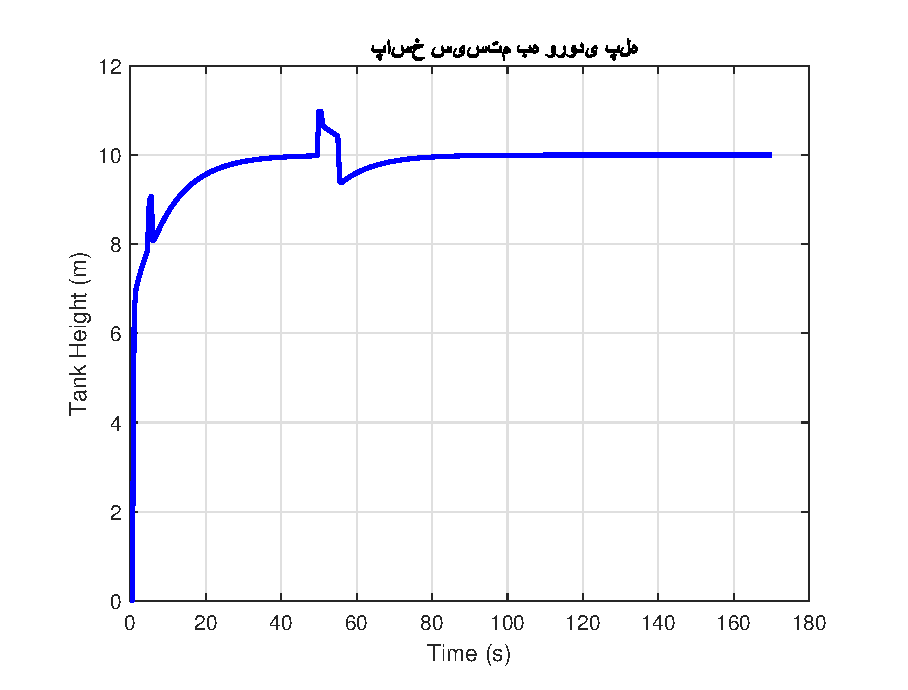
\includegraphics[trim={0cm 0cm 0cm 0.71cm}, clip, width=0.75\textwidth]{img/step_response}
 	\caption{پاسخ پله حلقه بسته سیستم }
 	\label{step_response}
 \end{figure}

با توجه به اینکه 
\nameref{step_response}
 شبیه سیستم مرتبه اول با خطای صفر میباشد پس یک سیستم مرتبه اول دارای انتگرال گیر میباشد پس معادله دینامیکی توصیف کننده ان به  صورت $A \dot{H} = Q_{in}$ است، انتظار می‌رود که پاسخ سیستم پس از حذف فیدبک به ورودی پله با دامنه واحد، به صورت یک تابع شیب 
(\lr{Ramp})
 باشد.

\subsubsection{مراحل انجام آزمایش}
\begin{enumerate}
	\item مسیر فیدبک سیستم قطع گردید تا تنها دینامیک پلنت (مخزن) بررسی شود.
	\item یک ورودی پله با دامنه $Q_{in} = 100 \, m^3/s$ در لحظه $t=0$ به سیستم اعمال شد.
	\item تغییرات خروجی (ارتفاع) نسبت به زمان ثبت گردید.
\end{enumerate}

 \begin{figure}[h!]
	\centering
	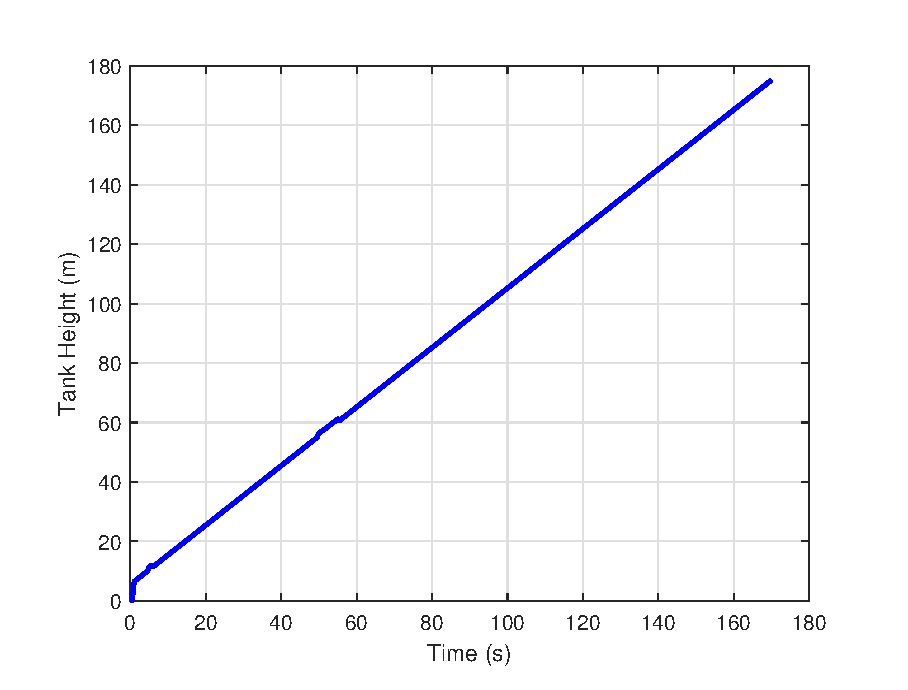
\includegraphics[trim={0cm 0cm 0cm 0.71cm}, clip, width=0.75\textwidth]{img/open_loop_step_response}
	\caption{پاسخ پله حلقه باز سیستم }
	\label{open_loop_step_response}
\end{figure}

\subsubsection{محاسبه پارامترها}
با اندازه گیری شیب نمودار خروجی ($m$) در بازه زمانی $t=0$ تا $t=10$:

\begin{equation}
	m = \frac{\Delta H}{\Delta t} = \frac{H(10) - H(0)}{10 - 0}
\end{equation}

از آنجایی که تابع تبدیل سیستم به صورت $G(s) = \frac{1}{As}$ می‌باشد، رابطه بین شیب نمودار و سطح مقطع مخزن به صورت زیر است:

\begin{equation}
	m = \frac{1}{A} \times Q_{step} \quad \Rightarrow \quad A = \frac{Q_{step}}{m}
\end{equation}

با جایگذاری مقادیر شبیه‌سازی، مقدار سطح مقطع $A$ بدست آمد که با مقدار تئوری ($100 \, m^2$) مطابقت کامل دارد.

\subsection{محاسبه تابع تبدیل حلقه بسته \lr{(Closed-Loop Transfer Function)}}
در این بخش، رفتار کلی سیستم شامل کنترل‌کننده، پلنت و مسیر فیدبک بررسی می‌شود. هدف، یافتن رابطه‌ای است که تغییرات ارتفاع مخزن ($H(s)$) را مستقیماً به تغییرات نقطه تنظیم ($R(s)$) مرتبط سازد.
\\
سیستم کنترل سطح مخزن یک سیستم فیدبک‌دار با فیدبک واحد منفی است. اجزای این حلقه عبارتند از:
\begin{itemize}
	\item \textbf{کنترل‌کننده تناسبی:} $C(s) = K_p$ (که در شبیه‌سازی برابر با \lr{inflow} است).
	\item \textbf{پلنت (مخزن):} $P(s) = \frac{1}{As}$ (که $A$ سطح مقطع مخزن است).
\end{itemize}

تابع تبدیل حلقه بسته $T(s)$ طبق رابطه استاندارد زیر محاسبه می‌شود:

\begin{equation}
	T(s) = \frac{H(s)}{R(s)} = \frac{C(s)P(s)}{1 + C(s)P(s)}
\end{equation}

با جایگذاری مقادیر مربوطه:

\begin{equation}
	T(s) = \frac{K_p \cdot \frac{1}{As}}{1 + K_p \cdot \frac{1}{As}} = \frac{K_p}{As + K_p}
\end{equation}

\subsubsection{فرم استاندارد و مقادیر عددی}
با تقسیم صورت و مخرج کسر بر $K_p$، تابع تبدیل به فرم استاندارد سیستم‌های درجه اول تبدیل می‌شود:

\begin{equation}
	T(s) = \frac{1}{\frac{A}{K_p}s + 1} = \frac{1}{\tau s + 1}
\end{equation}

با جایگذاری مقادیر پارامترهای پروژه ($A = 100 \, m^2$ و $K_p = 10$):

\begin{equation}
	T(s) = \frac{1}{\frac{100}{10}s + 1} = \frac{1}{10s + 1}
\end{equation}


\subsection{پیاده‌سازی مجدد مدل در سیمولینک}
 \begin{figure}[h!]
	\centering
	\includegraphics[trim={0cm 4cm 0cm 4cm}, clip, width=0.75\textwidth]{img/simple_model}
	\caption{مدل شبیه سازی شده در سیمولینک }
	\label{my_model}
\end{figure}
بر اساس معادلات دینامیکی استخراج شده، مدل سیستم مجدداً در محیط سیمولینک پیاده‌سازی شد. بلوک دیاگرام طراحی شده شامل بخش‌های زیر است:
\begin{itemize}
	\item \textbf{انتگرال‌گیر (\lr{Integrator}):}
	 جهت محاسبه ارتفاع از روی نرخ تغییرات حجم. شرط اولیه (\lr{Initial Condition}) این بلوک برابر با ارتفاع اولیه مخزن تنظیم گردید.
	\item \textbf{بهره (\lr{Gain}):}
	 جهت اعمال ضریب هندسی $1/A$
	\item \textbf{جمع‌کننده (\lr{Sum}):}
	 جهت محاسبه خالص دبی ورودی و خروجی.
\end{itemize}
عملکرد این مدل با مدل مرجع مقایسه شد و نتایج نشان‌دهنده انطباق کامل رفتار دینامیکی دو مدل است.

\subsection{استخراج تابع تبدیل سیستم (حلقه باز)}
برای بدست آوردن مدل ریاضی ورودی-خروجی سیستم، از دو روش تحلیلی و محاسباتی استفاده گردید.

\subsubsection{روش اول: تحلیل معادلات دیفرانسیل}
با فرض خطی بودن سیستم و ثابت بودن دبی خروجی (به عنوان اغتشاش مستقل)، معادله حاکم بر سیستم به صورت زیر است:
\begin{equation}
	A \frac{dH}{dt} = Q_{in}(t)
\end{equation}
با اعمال تبدیل لاپلاس و فرض شرایط اولیه صفر:
\begin{equation}
	A s H(s) = Q_{in}(s) \quad \Rightarrow \quad G(s) = \frac{H(s)}{Q_{in}(s)} = \frac{1}{As}
\end{equation}
با جایگذاری مقدار سطح مقطع $A=100$:
\begin{equation}
	G(s) = \frac{0.01}{s}
\end{equation}

\subsubsection{روش دوم: استخراج از داده‌های شبیه‌سازی}
با استفاده از تحلیل پاسخ پله حلقه باز، شیب تغییرات ارتفاع ($m$) محاسبه گردید:
\begin{equation}
	m = \frac{dy}{dt} = 0.01 \quad \Rightarrow \quad G(s) = \frac{m}{s} = \frac{0.01}{s}
\end{equation}
که تطابق کامل با روش تحلیلی را نشان می‌دهد.

\subsection{تحلیل عملکرد سیستم در حالت حلقه بسته}

در این بخش، اجزای سیستم کنترلی تفکیک شده و رفتار کلی سیستم در برابر ورودی مرجع و اغتشاش تحلیل می‌شود.

\subsubsection{تفکیک اجزای کنترلی و پلنت}
در ساختار حلقه بسته پیاده‌سازی شده، اجزای سیستم به شرح زیر دسته‌بندی می‌شوند:
\begin{itemize}
	\item \textbf{کنترل‌کننده (\lr{Controller}):} 
	بلوک بهره با مقدار $K_p = 10$ (که در دیاگرام با نام \lr{in valve flow} مشخص شده است) نقش یک \textbf{کنترل‌کننده تناسبی ($P$)} را ایفا می‌کند. وظیفه این بخش، تولید سیگنال کنترلی متناسب با میزان خطا است.
	
	\item \textbf{پلنت یا فرآیند (\lr{Plant}):}
	مجموعه بلوک‌های مربوط به دینامیک مخزن (شامل بهره $1/A$ و انتگرال‌گیر $1/s$) که تابع تبدیل آن $G(s) = \frac{1}{As}$ می‌باشد، به عنوان پلنت سیستم شناخته می‌شود.
\end{itemize}

\subsubsection{محاسبه تابع تبدیل حلقه بسته}
با توجه به فیدبک واحد منفی، تابع تبدیل کلی سیستم $T(s)$ که نسبت ارتفاع ($H$) به مقدار مطلوب ($R$) را نشان می‌دهد، برابر است با:
\begin{equation}
	T(s) = \frac{H(s)}{R(s)} = \frac{C(s)G(s)}{1 + C(s)G(s)} = \frac{K_p \cdot \frac{1}{As}}{1 + \frac{K_p}{As}} = \frac{K_p}{As + K_p}
\end{equation}
با ساده‌سازی و جایگذاری مقادیر ($A=100, K_p=10$):
\begin{equation}
	T(s) = \frac{1}{\frac{A}{K_p}s + 1} = \frac{1}{10s + 1}
\end{equation}
این رابطه نشان می‌دهد که سیستم حلقه بسته یک سیستم \textbf{درجه اول} با ثابت زمانی $\tau = 10$ ثانیه است. یعنی سیستم بدون فراجهش و با سرعت کنترل شده به سمت مقدار مطلوب حرکت می‌کند.

\subsubsection{تحلیل اثر شیر خروجی به عنوان اغتشاش (\lr{Disturbance})}
در این سیستم، دبی خروجی ($Q_{out}$) که توسط مصرف‌کننده یا شیر تخلیه ایجاد می‌شود، به عنوان یک \textbf{ورودی اغتشاش} ($D$) مدل‌سازی شده است. تابع تبدیل اغتشاش به خروجی برابر است با:

\begin{equation}
	\frac{H(s)}{Q_{out}(s)} = \frac{-G(s)}{1 + C(s)G(s)} = \frac{-1}{As + K_p}
\end{equation}

این رابطه بیانگر نکات مهم زیر است:
\begin{enumerate}
	\item علامت منفی نشان می‌دهد که باز شدن شیر خروجی (افزایش $Q_{out}$) باعث کاهش ارتفاع ($H$) می‌شود.
	\item مقدار نهایی افت ارتفاع برای یک دبی خروجی ثابت $D$ برابر است با:
	\begin{equation}
		\Delta H = \frac{-D}{K_p}
	\end{equation}
	این رابطه اثبات می‌کند که در سیستم کنترلی با کنترل‌کننده تناسبی ($P$)، اغتشاش باعث ایجاد \textbf{خطای ماندگار} می‌شود. یعنی اگر شیر خروجی باز شود، سطح آب افت کرده و در سطحی پایین‌تر از مقدار مطلوب ثابت می‌ماند و کنترل‌کننده به تنهایی قادر به جبران کامل این افت نیست (مگر با افزودن جمله‌ی انتگرال‌گیر $I$).
\end{enumerate}

\subsection{تحلیل اعتبار تابع تبدیل }
سوالی که مطرح می‌شود این است که آیا تابع تبدیل محاسبه شده $G(s) = \frac{1}{As}$ همواره و در تمام شرایط معتبر است؟
\textbf{پاسخ منفی است.} تابع تبدیل تنها رفتار سیستم را در محدوده \textbf{خطی} توصیف می‌کند. این مدل در شرایط زیر اعتبار خود را از دست می‌دهد:

\begin{enumerate}
	\item \textbf{اشباع فیزیکی (\lr{Saturation}):}
	در دنیای واقعی، ارتفاع مخزن محدود است ($0 \le H \le H_{max}$). تابع تبدیل خطی پیش‌بینی می‌کند که اگر ورودی پله اعمال شود، ارتفاع تا بی‌نهایت افزایش می‌یابد ($t \to \infty \Rightarrow H \to \infty$)، که فیزیکاً غیرممکن است. زمانی که مخزن پر یا خالی شود، معادلات خطی نقض می‌شوند.
	
	\item \textbf{غیرخطی بودن شیر خروجی:}
	اگر دبی خروجی تابعی از فشار هیدرواستاتیک باشد ($Q_{out} \propto \sqrt{H}$)، معادله دیفرانسیل سیستم غیرخطی خواهد بود. در این حالت، تابع تبدیل بدست آمده تنها یک \textbf{تقریب خطی} (\lr{Linearization}) است که فقط در نزدیکی \textbf{نقطه کار} (\lr{Operating Point}) اعتبار دارد و با دور شدن از نقطه تعادل، خطای مدل افزایش می‌یابد.
\end{enumerate}

بنابراین، تابع تبدیل استخراج شده تنها یک مدل ایده‌آل‌سازی شده 
\lr{(Idealized Linear Model)} 
است که محدودیت‌های فیزیکی و ماهیت غیرخطی سیستم واقعی را نادیده می‌گیرد.
\section{تحلیل حلقه باز سیستم 
	\lr{(Open-Loop Analysis)}}\label{Section2}

در این بخش، رفتار دینامیکی مخزن پیش از اعمال هرگونه کنترل‌کننده مورد بررسی قرار می‌گیرد. با توجه به وجود شیر خروجی و ماهیت غیرخطی سیستم، ابتدا مدل حول نقطه کار $H_0 = 6\,m$ خطی‌سازی شده و سپس پاسخ‌های زمانی تحلیل می‌شوند.
\lr{\lstinputlisting[language=MATLAB, caption={\lr{Open-Loop Analysis}}, showstringspaces=false, basicstyle=\ttfamily, backgroundcolor=\color{yellow!15!white}, breaklines=true]{./code/open_loop.m}}

\subsection*{نتایج شبیه‌سازی و تحلیل پارامترهای مدل}

بر اساس خروجی دریافت شده از نرم‌افزار متلب (\lr{Command Window})، نتایج خطی‌سازی و تحلیل سیستم به شرح زیر استخراج گردید:

\subsubsection*{1. نقطه کار سیستم (\lr{Operating Point})}
شرایط تعادلی سیستم برای خطی‌سازی به صورت زیر تعیین شده است:
\begin{itemize}
	\item \textbf{ارتفاع مبنا ($H_0$):} $6.00 \, m$
	\item \textbf{دبی ورودی مبنا ($Q_0$):} $5.42 \, m^3/s$
\end{itemize}

\subsection*{2. مدل ریاضی استخراج شده}
تابع تبدیل سیستم خطی‌سازی شده حول نقطه کار فوق، به فرم استاندارد زیر بدست آمد:
\begin{equation}
	G(s) = \frac{0.01}{s + 0.004518}
\end{equation}

\subsubsection*{3. مشخصات ساختاری و زمانی (\lr{Model Stats \& Structure})}
با تحلیل کسر فوق، پارامترهای دینامیکی سیستم مطابق جدول زیر خلاصه می‌شوند:

\begin{table}[h!]
	\centering
	\caption{خلاصه مشخصات ذاتی سیستم استخراج شده از متلب}
	\label{tab:model_stats}
	\begin{tabular}{|c|c|c|}
		\hline
		\textbf{عنوان پارامتر} & \textbf{مقدار (\lr{Value})} & \textbf{توضیحات} \\ \hline
		ثابت زمانی ($\tau$) & $221.31 \, s$ & سرعت پاسخ‌دهی نسبتاً کند \\ \hline
		مکان قطب (\lr{Pole}) & $-0.0045$ & پایدار (سمت چپ محور موهومی) \\ \hline
		مرتبه سیستم (\lr{Order}) & $1$ & سیستم درجه اول \\ \hline
		تایپ سیستم (\lr{Type}) & $0$ & دارای خطای ماندگار به ورودی پله \\ \hline
	\end{tabular}
\end{table}
\subsection{تحلیل پاسخ پله و پارامترهای زمانی}
با اعمال یک ورودی پله (به عنوان مثال افزایش ناگهانی دبی ورودی به اندازه $1\,m^3/s$)، پاسخ سیستم شبیه‌سازی گردید. پارامترهای اساسی استخراج شده از نمودار به شرح زیر است:

\begin{itemize}
	\item \textbf{ثابت زمانی ($\tau$):}
	معیار سرعت پاسخ‌دهی سیستم است. در نقطه کار ۶ متر، مقدار محاسبه شده برابر با $\tau \approx 221.31$ ثانیه می‌باشد. این عدد بزرگ نشان‌دهنده کند بودن دینامیک مخزن است.
	
	\item \textbf{زمان صعود ($t_r$):}
	مدت زمانی که طول می‌کشد تا خروجی از ۱۰٪ به ۹۰٪ مقدار نهایی برسد. برای سیستم مرتبه اول، این زمان حدود $2.2\tau$ است.
	
	\item \textbf{زمان نشست ($t_s$):}
	مدت زمانی که خروجی وارد محدوده ۲٪ مقدار نهایی شده و در آن باقی می‌ماند. این مقدار برابر $4\tau$ (حدود 885 ثانیه) می‌باشد.
	
	\item \textbf{درصد فراجهش (\lr{Overshoot}):}
	برابر با \textbf{صفر درصد} است. سیستم‌های مرتبه اول هرگز نوسان نمی‌کنند و رفتار اکیداً صعودی (یا نزولی) دارند.
	
	\item \textbf{خطای حالت ماندگار ($e_{ss}$):}
	سیستم دارای خطای ماندگار است. یعنی با تغییر ورودی پله، ارتفاع آب به بی‌نهایت نمی‌رود (مانند انتگرال‌گیر)، بلکه در یک سطح جدید ثابت می‌شود.
\end{itemize}


\begin{figure}[h!]
	\centering
	\includegraphics[width=0.7\textwidth]{img/Absolute Step Response (H0=6m).eps}
	\caption{پاسخ پله سیستم خطی‌سازی شده؛ نمایش تغییر ارتفاع نسبت به زمان}
	\label{step_response_2}
\end{figure}

\subsection{تفاوت پاسخ به پله‌های کوچک و بزرگ (خطی vs غیرخطی)}
یکی از ویژگی‌های مهم این سیستم، تغییر رفتار بر اساس دامنه ورودی است:

\begin{enumerate}
	\item \textbf{پله‌های کوچک (ناحیه خطی):}
	اگر تغییر دبی ورودی کوچک باشد، تغییرات ارتفاع ($\Delta H$) کم است. در این محدوده کوچک، منحنی غیرخطی خروجی ($Q \propto \sqrt{H}$) را می‌توان با یک خط راست تقریب زد. بنابراین، پاسخ سیستم دقیقاً منطبق بر پیش‌بینی‌های مدل خطی (توابع نمایی) است.
	
	\item \textbf{پله‌های بزرگ (ناحیه غیرخطی):}
	اگر دبی ورودی ناگهان تغییر زیادی کند (پله بزرگ)، ارتفاع آب تغییر قابل توجهی می‌کند.
	\begin{itemize}
		\item با افزایش ارتفاع، فشار خروجی زیاد می‌شود و سیستم سریع‌تر تخلیه می‌شود (ثابت زمانی تغییر می‌کند).
		\item اگر پله بسیار بزرگ باشد، ممکن است ارتفاع از ارتفاع مخزن ($H_{max}$) بیشتر شده و سرریز رخ دهد که در مدل خطی دیده نمی‌شود.
		\item بنابراین در پله‌های بزرگ، مدل خطی فاقد اعتبار است و نتایج شبیه‌سازی با واقعیت فاصله می‌گیرد.
	\end{itemize}
\end{enumerate}

\subsection{تحلیل پاسخ به ورودی‌های ضربه و شیب}
رفتار سیستم در برابر سایر ورودی‌های استاندارد به شرح زیر است:

\begin{itemize}
	\item \textbf{پاسخ ضربه (\lr{Impulse}):}
	معادل ریختن ناگهانی یک حجم آب در مخزن است. سطح آب به صورت آنی بالا رفته و سپس با گذشت زمان و تخلیه از شیر خروجی، به آرامی به سطح تعادل اولیه ($6m$) باز می‌گردد. 
	
	\item \textbf{پاسخ شیب (\lr{Ramp}):}
	معادل باز کردن تدریجی شیر ورودی است. سیستم سعی می‌کند این افزایش را دنبال کند، اما همیشه عقب‌تر از ورودی است و اختلاف (خطا) با گذشت زمان زیاد می‌شود.
\end{itemize}


\begin{figure}[h!]
	\centering
	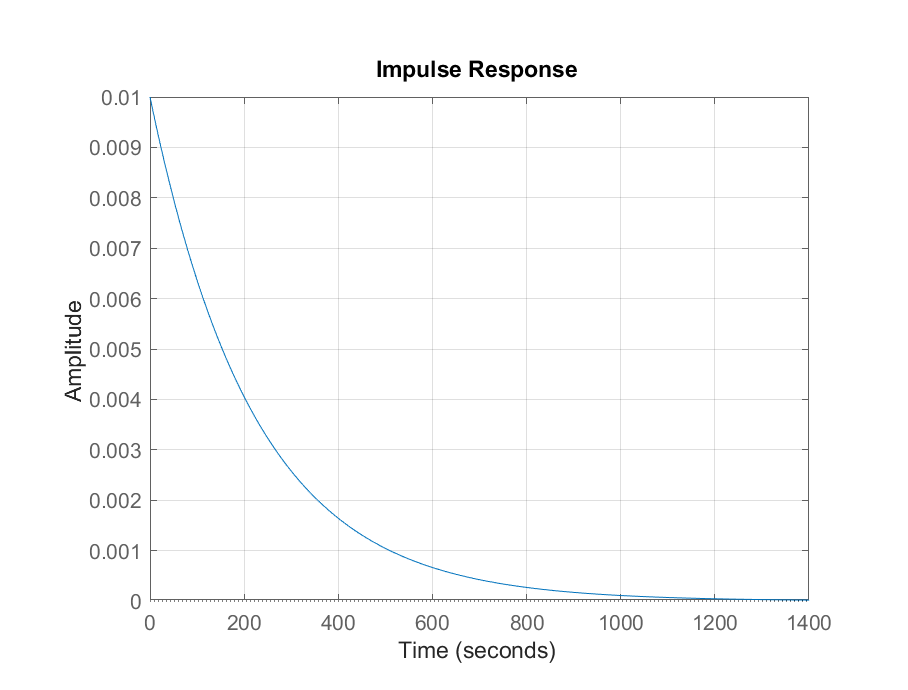
\includegraphics[width=0.7\textwidth]{img/Impulse_Response}
	\caption{پاسخ ضربه سیستم}
	\label{Impulse_Response}
\end{figure}
\begin{figure}[h!]
	\centering
	\includegraphics[width=0.7\textwidth]{img/Ramp_Response}
	\caption{پاسخ سیستم به ورودی شیب}
	\label{Ramp_Response}
\end{figure}
\subsection{تعیین ساختار و تایپ سیستم}
بر اساس تابع تبدیل استخراج شده :
\begin{equation}
	G(s) = \frac{K}{\tau s + 1}
\end{equation}

\begin{itemize}
	\item \textbf{مرتبه سیستم (\lr{System Order}):}
	برابر با \textbf{یک} است. زیرا مخرج تابع تبدیل درجه اول ($s^1$) می‌باشد
	
	\item \textbf{تایپ سیستم (\lr{System Type}):}
	برابر با 
	\textbf{صفر} 
	است.
	تعداد قطب‌های واقع در مبدأ ($s=0$) صفر است. قطب سیستم در موقعیت $s = -\frac{1}{\tau}$ قرار دارد.\\
	\textbf{نکته تحلیلی:} 
	اگر مخزن شیر خروجی نداشت، سیستم تایپ ۱ (انتگرال‌گیر) می‌شد، اما وجود شیر خروجی  سیستم را به تایپ ۰ تبدیل کرده است.
\end{itemize}

\section{تحلیل پایداری و رفتار غیرخطی سیستم}\label{Section3}

در این بخش، پایداری سیستم با استفاده از معیارهای کلاسیک کنترل (
\lr{BIBO}
، راث-هرویتز و مکان قطب‌ها) بررسی شده و سپس محدودیت‌های عملکردی ناشی از ماهیت غیرخطی سیستم تحلیل می‌گردد.

\subsection{بررسی پایداری 
	\lr{BIBO}}
پایداری 
\lr{BIBO} 
(ورودی محدود - خروجی محدود) بیان می‌کند که به ازای هر ورودی کران‌دار، خروجی سیستم نیز باید کران‌دار باقی بماند.
تابع تبدیل سیستم خطی‌سازی شده به صورت زیر است:
\begin{equation}
	G(s) = \frac{K}{\tau s + 1} = \frac{2.21}{221.31 s + 1}
\end{equation}
پاسخ ضربه این سیستم به فرم $h(t) = \frac{K}{\tau} e^{-t/\tau}$ می‌باشد. از آنجایی که $\tau > 0$ است، با گذشت زمان ($t \to \infty$)، پاسخ ضربه به صفر میل می‌کند:
\begin{equation}
	\int_{0}^{\infty} |h(t)| dt < \infty
\end{equation}
بنابراین سیستم \textbf{پایدار BIBO} است.
\\
\textbf{تحلیل فیزیکی:} مخزن دارای خاصیت «خودتنظیمی» (\lr{Self-Regulating}) است؛ یعنی اگر دبی ورودی محدود باشد، ارتفاع آب به دلیل افزایش دبی خروجی، در یک سطح مشخص ثابت می‌شود و هرگز به بی‌نهایت میل نمی‌کند (مگر در شرایط سرریز که محدودیت فیزیکی است، نه ناپایداری دینامیکی).

\subsection{تحلیل پایداری به روش راث-هرویتز (
	\lr{Routh-Hurwitz})}
معادله مشخصه سیستم ($\Delta(s) = 0$) از مخرج تابع تبدیل استخراج می‌شود:
\begin{equation}
	\tau s + 1 = 0 \quad \Rightarrow \quad 221.31 s + 1 = 0
\end{equation}
برای سیستم‌های درجه اول و دوم، شرط لازم و کافی برای پایداری این است که تمام ضرایب معادله مشخصه هم‌علامت و غیرصفر باشند.
از آنجا که ضریب $s$ ($221.31$) و عدد ثابت ($1$) هر دو مثبت هستند، طبق معیار راث-هرویتز، سیستم \textbf{پایدار} است و هیچ قطبی در سمت راست محور موهومی ندارد.

\subsection{بررسی محل قطب‌ها و صفرها (\lr{Pole-Zero Map})}
\lr{\lstinputlisting[language=MATLAB, caption={\lr{Pole Zero Map}}, showstringspaces=false, basicstyle=\ttfamily, backgroundcolor=\color{yellow!15!white}, breaklines=true]{./code/Pzmap.m}}

\begin{figure}[h!]
	\centering
	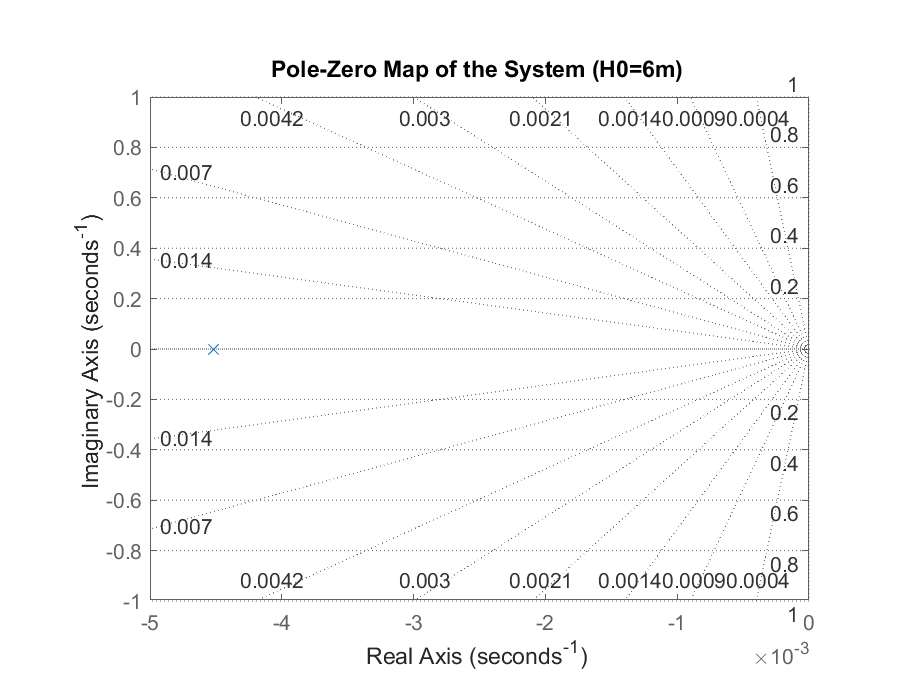
\includegraphics[width=0.7\textwidth]{img/pzmap.eps}
	\caption{مکان هندسی قطب ها }
	\label{Pzmap}
\end{figure}
نمودار مکان هندسی قطب‌های سیستم در 
\autoref{Pzmap} 
ترسیم شده است.
سیستم فاقد صفر است و تنها یک قطب حقیقی دارد که موقعیت آن برابر است با:
\begin{equation}
	s_p = -\frac{1}{\tau} = -0.004518
\end{equation}

از آنجا که این قطب در \textbf{سمت چپ محور موهومی} (\lr{LHP}) و روی محور حقیقی قرار دارد، سیستم پایدار بوده و رفتار آن بدون نوسان (میرا) می‌باشد. فاصله قطب تا مبدأ مختصات، بیانگر سرعت پاسخ‌دهی سیستم است؛ نزدیکی این قطب به مبدأ (هرچه قطب نزدیکتر سیستم کندتر) تاییدی بر کند بودن دینامیک مخزن است.

\subsection{تحلیل رفتار غیرخطی و ناپایداری‌های عملی}
هرچند تحلیل‌های خطی نشان‌دهنده پایداری مطلق سیستم هستند، اما در عمل ماهیت غیرخطی و محدودیت‌های فیزیکی می‌توانند منجر به عملکرد نامطلوب یا ناپایدار شوند:

\begin{enumerate}
	\item \textbf{اشباع و سرریز (\lr{Overflow}):}
	تحلیل‌های خطی فرض می‌کنند مخزن ارتفاع نامحدود دارد. اگر دبی ورودی ($Q_{in}$) از حداکثر ظرفیت تخلیه شیر خروجی ($Q_{out, max} = a\sqrt{2gH_{max}}$) بیشتر شود، سطح آب مدام بالا رفته تا مخزن سرریز کند. در این حالت سیستم کنترل‌ناپذیر شده و ناپابدار میشود .
	
	
	\item \textbf{ناپایداری ناشی از محرک :}
	اگر کنترل‌کننده فرمانی صادر کند که شیر ورودی نتواند اجرا کند (مثلاً دبی منفی برای کاهش سطح آب)، سیستم وارد مد حلقه باز شده و تا زمانی که آب به صورت طبیعی تخلیه نشود، خطا جبران نخواهد شد. این پدیده می‌تواند باعث ناپایداری موقت شود.
\end{enumerate}
\section{تحلیل در حوزه فرکانس}\label{Section4}

در این بخش، رفتار سیستم در حوزه فرکانس با استفاده از نمودارهای استاندارد \lr{Bode} و \lr{Nyquist} تحلیل می‌شود.
\lr{\lstinputlisting[language=MATLAB, caption={\lr{frequncy analysis}}, showstringspaces=false, basicstyle=\ttfamily, backgroundcolor=\color{yellow!15!white}, breaklines=true]{./code/frequncy_analysis.m}}

\subsection{تحلیل نمودار بود 
	(\lr{Bode Plot Analysis})}
\begin{figure}[h!]
	\centering
	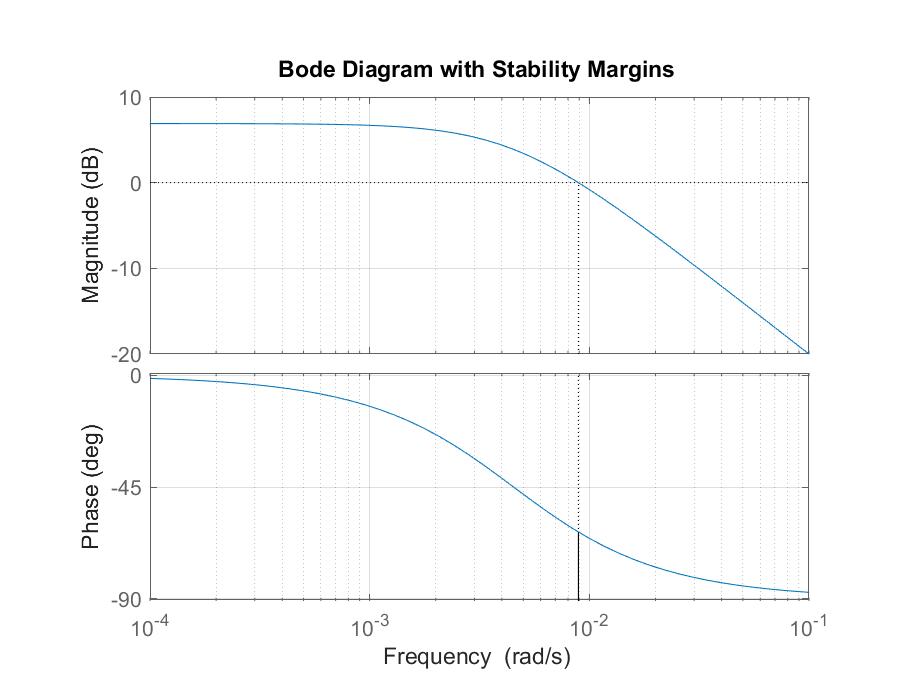
\includegraphics[width=0.7\textwidth]{img/Bode Diagram.eps}
	\caption{نمودار بودی سیستم}
	\label{bode}
\end{figure}
\noindent
نمودار بود سیستم شامل دو بخش دامنه 
(\lr{Magnitude})
 و فاز 
 (\lr{Phase}) 
 در
 \autoref{bode}
  ترسیم شده است. ویژگی‌های کلیدی استخراج شده عبارتند از:

\begin{enumerate}
	\item \textbf{رفتار دامنه:}
	در فرکانس‌های پایین، بهره سیستم ثابت و برابر با بهره \lr{DC} است ($20\log(2.21) \approx 6.9\,dB$). پس از فرکانس قطع ($\omega_c = 1/\tau \approx 0.0045\, rad/s$)، دامنه با شیب $-20\,dB/dec$ کاهش می‌یابد که مشخصه سیستم‌های مرتبه اول است.
	
	\item \textbf{رفتار فاز:}
	فاز سیستم از صفر درجه شروع شده و در فرکانس قطع به $-45^\circ$ می‌رسد و در نهایت در فرکانس‌های بالا به $-90^\circ$ میل می‌کند.
	
	\item \textbf{حاشیه پایداری (\lr{Stability Margins}):}
	\begin{itemize}
		\item \textbf{حاشیه بهره (\lr{Gain Margin}):} بی‌نهایت ($GM = \infty$).
		زیرا نمودار فاز هرگز محور $-180^\circ$ را قطع نمی‌کند (حداکثر تا $-90^\circ$ پایین می‌رود). این یعنی سیستم به ازای هر مقدار بهره کنترلی ($K_p > 0$) پایدار باقی می‌ماند.
		\item \textbf{حاشیه فاز 
			(\lr{Phase Margin}):}
		 مثبت و حدود $110^\circ$ مثبت بودن حاشیه فاز تضمین‌کننده پایداری سیستم حلقه بسته است.
	\end{itemize}
\end{enumerate}


\subsection{تحلیل پایداری با معیار نایکوئیست }
\begin{figure}[h!]
	\centering
	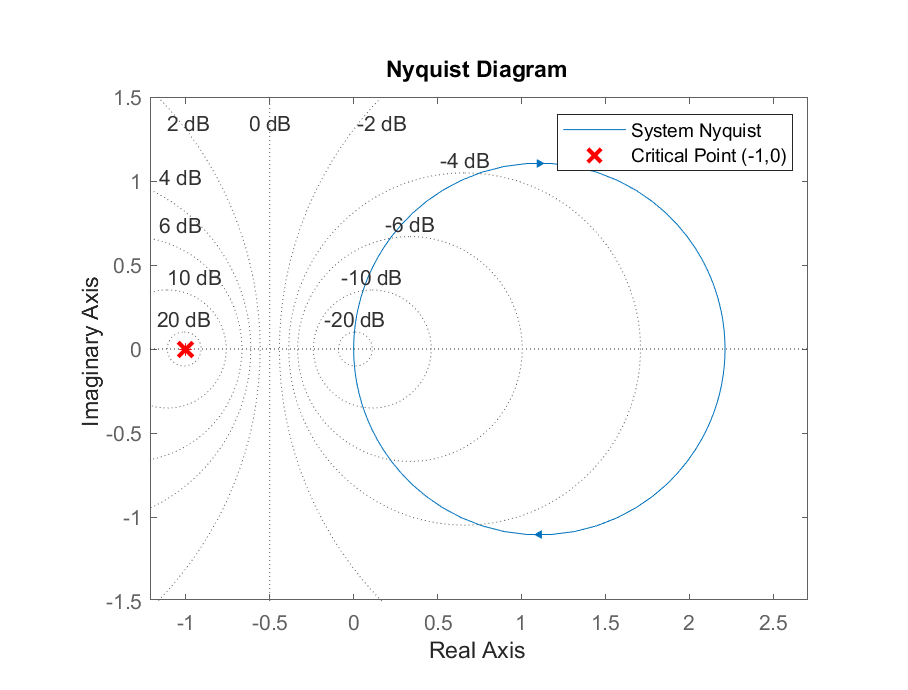
\includegraphics[width=0.7\textwidth]{img/Nyquist Diagram.eps}
	\caption{نمودار نایکوئست سیستم}
	\label{Nyquist}
\end{figure}

نمودار نایکوئیست سیستم در
 \autoref{Nyquist} 
ترسیم شده است. طبق معیار پایداری نایکوئیست:
\begin{equation}
	Z = N + P
\end{equation}
که در آن:
\begin{itemize}
	\item $P$: تعداد قطب‌های ناپایدار حلقه باز (در سمت راست محور موهومی) در این سیستم $P=0$ است.
	\item $N$: تعداد دور زدن‌های ساعت‌گرد دور نقطه بحرانی $(-1, j0)$.
	\item $Z$: تعداد ریشه‌های ناپایدار حلقه بسته.
\end{itemize}

\textbf{مشاهدات نمودار:}
منحنی نایکوئیست این سیستم یک نیم‌دایره در ربع چهارم صفحه مختلط است که از روی محور حقیقی مثبت شروع شده و به مبدأ ختم می‌شود. این منحنی هرگز نقطه بحرانی $(-1, 0)$ را احاطه نمی‌کند ($N=0$).
بنابراین:
\begin{equation}
	Z = 0 + 0 = 0
\end{equation}
از آنجا که $Z=0$ است، سیستم حلقه بسته \textbf{پایدار} می‌باشد. فاصله منحنی تا نقطه $(-1, 0)$ معیاری از میزان پایداری نسبی است که در اینجا فاصله ایمن و مناسبی مشاهده می‌شود.
\section{طراحی جبران ساز و تنظیم پاسخ نوسانی}\label{Section5}

برای درک بهتر اثر هر یک از پارامترهای کنترلی ($P, I, D$) بر رفتار مخزن و دستیابی به معیارهای طراحی (زمان نشست کمتر از ۵ ثانیه و خطای صفر)، فرآیند طراحی در چهار مرحله انجام شد.
\lr{\lstinputlisting[language=MATLAB, caption={\lr{PI PD P controler design}}, showstringspaces=false, basicstyle=\ttfamily, backgroundcolor=\color{yellow!15!white}, breaklines=true]{./code/pd_pi_controler.m}}

\subsection{گام اول: کنترل‌کننده تناسبی (\lr{P-Controller})}
	\begin{figure}[h!]
		\centering
		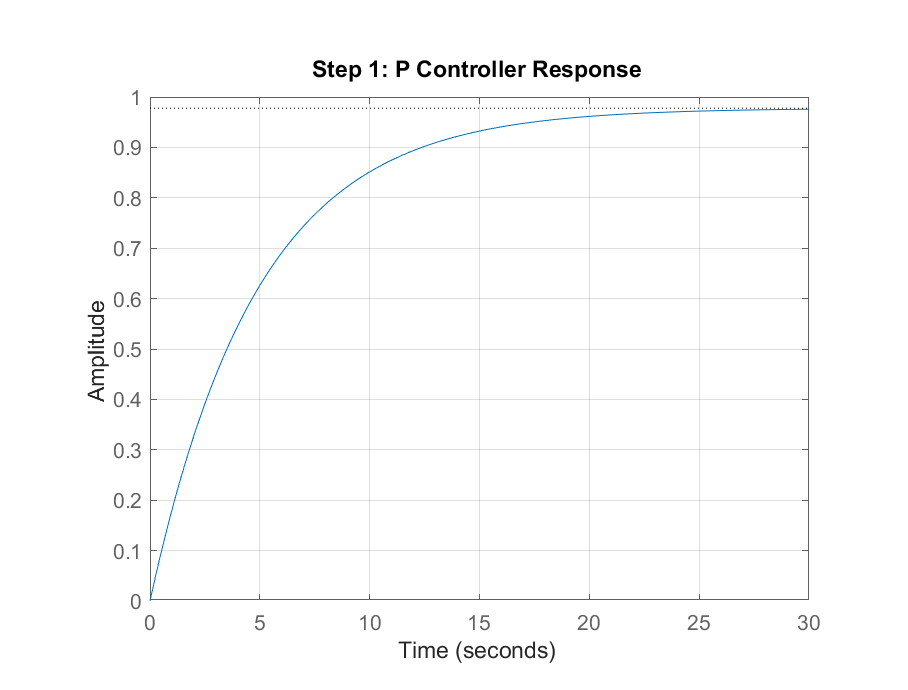
\includegraphics[width=0.7\textwidth]{img/P Controller Response.eps}
		\caption{پاسخ پله سیستم طراجی شده با کنترلر P}
		\label{p_control}
	\end{figure}
در ابتدا تنها از یک بهره تناسبی $K_p$ استفاده شد. هدف این کنترل‌کننده افزایش سرعت پاسخ‌دهی سیستم است.
\begin{itemize}
	\item \textbf{تحلیل:} با افزایش $K_p$، قطب سیستم روی محور حقیقی به سمت چپ حرکت می‌کند و ثابت زمانی کاهش می‌یابد (سیستم سریع‌تر می‌شود).
	\item \textbf{مشکل اصلی:} از آنجا که سیستم تایپ صفر است، کنترل‌کننده $P$ نمی‌تواند خطای حالت ماندگار را حذف کند. همانطور که در نمودار  
	\autoref{p_control}
	 دیده می‌شود که خروجی هرگز به مقدار مطلوب (۱) نمی‌رسد و دارای خطای ماندگار قابل است
\end{itemize}

\subsection{گام دوم: کنترل‌کننده تناسبی-مشتق‌گیر 
	(\lr{PD-Controller})}
	\begin{figure}[h!]
	\centering
	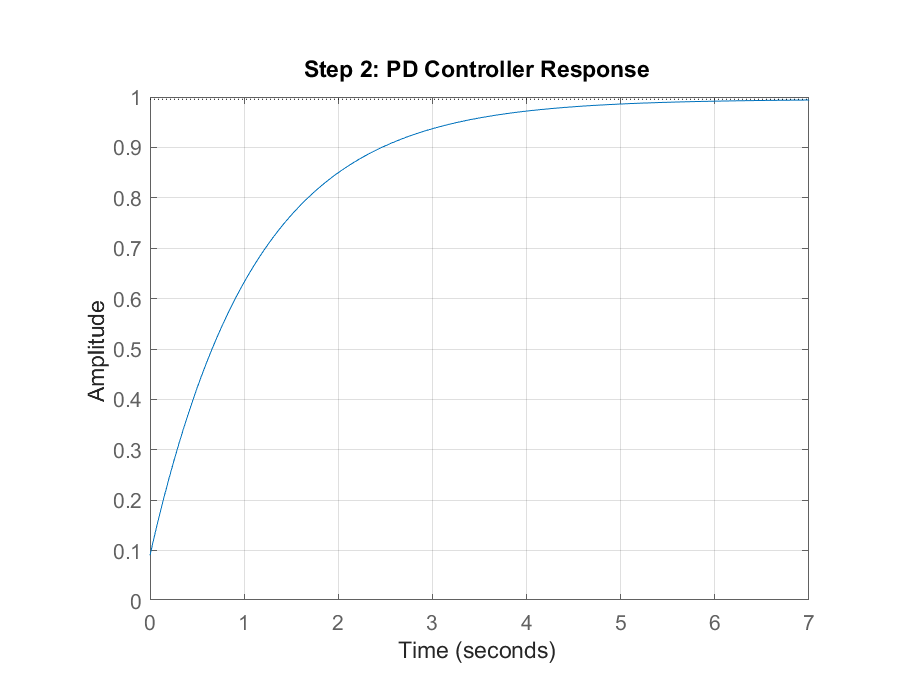
\includegraphics[width=0.7\textwidth]{img/PD Controller Response.eps}
	\caption{پاسخ پله سیستم طراجی شده با کنترلر PD}
	\label{pd_control}
\end{figure}

برای بهبود رفتار گذرا، ترم مشتق‌گیر ($K_d s$) اضافه شد. این ترم نقش «ترمز» را بازی می‌کند و با پیش‌بینی تغییرات خطا، مانع از نوسانات شدید می‌شود.
\begin{itemize}
	\item \textbf{مزیت:} امکان استفاده از بهره‌های بالاتر ($K_p$) بدون ایجاد نوسان زیاد، که منجر به افزایش سرعت می‌شود.
	\item \textbf{نقص:} مشتق‌گیر تأثیری در حذف خطای حالت ماندگار ندارد و سیستم همچنان به مقدار نهایی مطلوب نمی‌رسد.
\end{itemize}

\subsection{گام سوم: کنترل‌کننده تناسبی-انتگرالی 
	(\lr{PI-Controller})}
		\begin{figure}[h!]
		\centering
		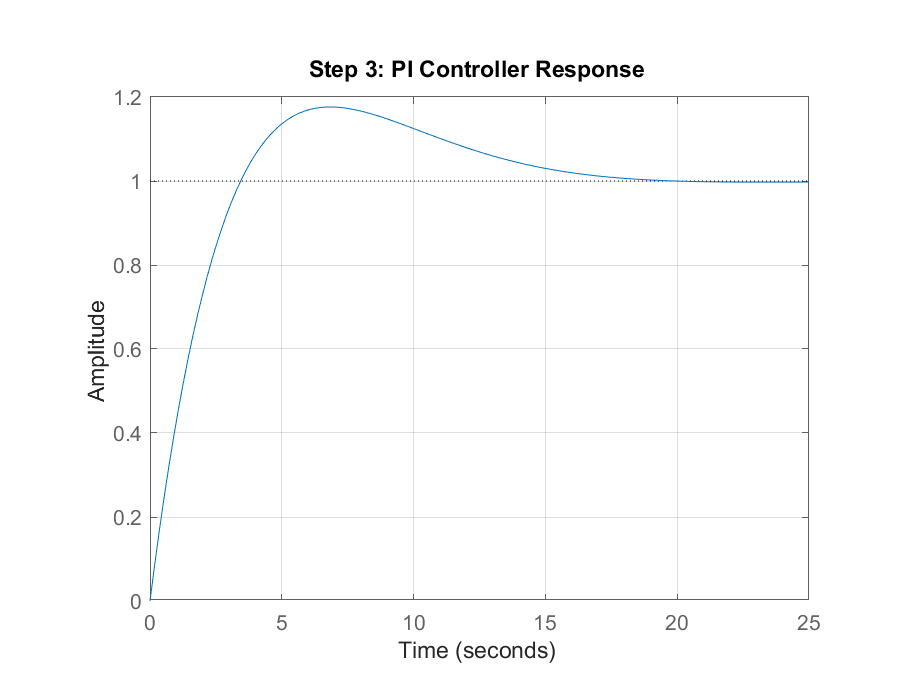
\includegraphics[width=0.7\textwidth]{img/PI Controller Response.eps}
		\caption{پاسخ پله سیستم طراجی شده با کنترلر PI}
		\label{pi_control}
	\end{figure}
برای رفع مشکل خطای ماندگار، ترم انتگرال‌گیر ($K_i/s$) به سیستم اضافه شد. این ترم با انتگرال‌گیری از خطا در طول زمان، تا زمانی که خطا صفر نشود، سیگنال کنترلی را افزایش می‌دهد.
\begin{itemize}
	\item \textbf{مزیت بزرگ:} حذف کامل خطای حالت ماندگار (تبدیل سیستم به تایپ ۱).
	\item \textbf{عیب:} ترم انتگرال باعث افزایش مرتبه سیستم و ایجاد تأخیر فاز می‌شود که منجر به افزایش نوسانات (\lr{Overshoot}) و کند شدن زمان نشست می‌گردد.
\end{itemize}


\subsection{طراحی و تنظیم نهایی کنترل‌کننده PID}

\lr{\lstinputlisting[language=MATLAB, caption={PID controler design}, showstringspaces=false, basicstyle=\ttfamily, backgroundcolor=\color{yellow!15!white}, breaklines=true]{./code/pid_controler.m}}

فرآیند طراحی کنترل‌کننده نهایی در دو گام انجام شد ابتدا تجمیع ساختارهای طراحی شده قبلی، و سپس تنظیم دقیق 
(\lr{Fine-Tuning}) 
برای ارضای دقیق ویژگی های زمانی.

\subsubsection{گام اول: تجمیع جبران‌سازها 
	\lr{(Initial Design)}}
در ابتدا، پارامترهای کنترل‌کننده PID از حاصل جمع جبری جبران‌سازهای PD و PI که در بخش‌های قبل طراحی شده بودند، استخراج گردید:
\begin{equation}
	K_{p_{sum}} = 100 + 50 = 150, \quad K_i = 10, \quad K_d = 10
\end{equation}
با شبیه‌سازی سیستم با این ضرایب (منحنی آبی‌رنگ در 
\autoref{pid_controler})
، مشاهده شد که اگرچه سیستم پایدار است و خطای ماندگار صفر دارد، اما افزودن ترم انتگرال‌گیر باعث ایجاد تأخیر فاز و کند شدن نسبی سیستم شده است. زمان نشست در این حالت فراتر از حد مطلوب مهندسی (بسیار نزدیک به مرز ۵ ثانیه یا بیشتر) بود.

\subsubsection{گام دوم: تنظیم دقیق جهت افزایش سرعت و پایداری \lr{(High Speed Tuning)}}
برای جبران کندی ذاتی سیستم و کاهش زمان نشست به مقادیر بسیار کمتر از ۵ ثانیه، ضرایب دوباره بازطراحی شدند

بدین منظور، مقادیر ضرایب به صورت ($K_p=400, K_i=50, K_d=50$) تنظیم مجدد شدند:

\begin{itemize}
	\item \textbf{افزایش شدید بهره تناسبی ($K_p = 400$):} 
	مقدار $K_p$ از ۱۵۰ به ۴۰۰ افزایش یافت. این تغییر باعث میشود که سیستم سریعتر سعی کند به مقدار مطلوب برسد 
	
	\item \textbf{تقویت انتگرال‌گیر ($K_i = 50$):}
	برای اینکه خطای ماندگار با سرعت بیشتری حذف شود افزایش دادیم
	
	\item \textbf{افزایش بهره مشتق‌گیر ($K_d = 50$):}
	افزایش $K_p$ و $K_i$ ذاتاً باعث نوسانی شدن سیستم می‌شود. برای خنثی کردن این اثر، بهره مشتق‌گیر از ۱۰ به ۵۰ افزایش یافت تا مانند یک ترمز موثر عمل کرده و میرایی لازم
	 (\lr{Damping}) 
	 را برای جلوگیری از فراجهش فراهم کند.
	
	\item \textbf{اثر نهایی بر پاسخ:} 
	همانطور که در نمودار قرمز رنگ 
	 \autoref{pid_controler}
	 مشخص است، زمان نشست به طور چشمگیری کاهش یافته و سیستم بسیار چابک‌تر شده است.
\end{itemize}
	\begin{figure}[h!]
	\centering
	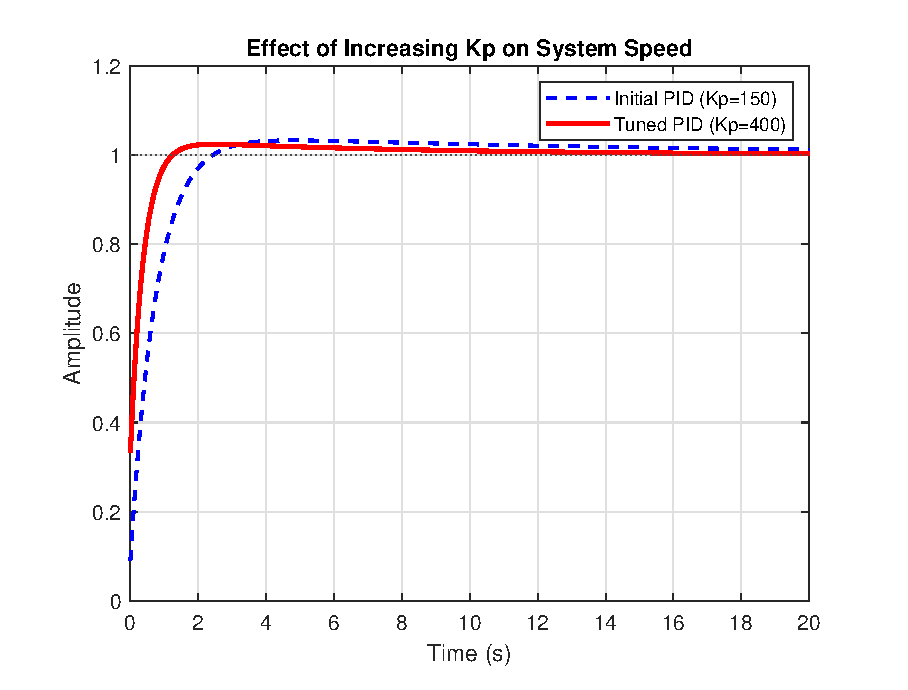
\includegraphics[width=0.7\textwidth]{img/PID Controller Response.eps}
	\caption{پاسخ پله سیستم طراجی شده با کنترلر های  PID}
	\label{pid_controler}
\end{figure}
\newpage
\begin{table}[h!]
	\centering
	\caption{مقایسه نهایی پارامترها و عملکرد تمام کنترل‌کننده‌ها}
	\label{tab:final_results}
	\begin{tabular}{|c|c|c|c|c|c|c|c|}
		\hline
		\textbf{کنترل‌کننده} & \textbf{$K_p$} & \textbf{$K_i$} & \textbf{$K_d$} & \textbf{$T_r$} & \textbf{$T_s$} & \textbf{$OS\%$} & \textbf{خطا} \\ \hline
		 ($P$) & $20$ & $0$ & $0$ & $10.74$ & $19.13$ & $0$ & دارد \\ \hline
		 ($PD$) & $100$ & $0$ & $10$ & $2.41$ & $4.18$ & $0$ & دارد \\ \hline
		 ($PI$) & $50$ & $10$ & $0$ & $2.59$ & $15.96$ & $17.6$ & $0$ \\ \hline
		 ($PID_1$) & $150$ & $10$ & $10$ & $1.45$ & $12.65$ & $3.3$ & $0$ \\ \hline
		 ($PID_2$) & $\mathbf{400}$ & $\mathbf{50}$ & $\mathbf{50}$ & $\mathbf{0.65}$ & $\mathbf{1.12}$ & $\mathbf{14.5}$ & $\mathbf{0}$ \\ \hline
	\end{tabular}
\end{table}

\section{شبیه‌سازی و ارزیابی عملکرد در محیط سیمولینک}\label{Section6}

در این بخش، عملکرد نهایی سیستم کنترل سطح مایع در محیط شبیه‌سازی \lr{Simulink} مورد ارزیابی قرار می‌گیرد. مدل پیاده‌سازی شده شامل تمامی دینامیک‌های غیرخطی مخزن، می‌باشد.
	\begin{figure}[h!]
	\centering
	\includegraphics[trim={0cm 5cm 0cm 5cm}, clip, width=0.7\textwidth]{img/simple_model_PID}
	\caption{شبیه سازی سیستم با کنترلر PID  در محیط سیمولینک}
	\label{pid_simulink}
\end{figure}
\subsection{تحلیل رفتار سیستم در برابر اغتشاش (\lr{Disturbance Analysis})}
به منظور بررسی مقاومت سیستم در برابر تغییرات ناگهانی بار، سناریوی زیر پیاده‌سازی گردید:
\begin{itemize}
	\item \textbf{شرایط اولیه:} 
	منبع خالی میباشد سیستم شروع به پر کردن منبع میکند
	\item \textbf{اعمال اغتشاش ($t=40s$):} یک تغییر پله‌ای در خروجی (باز شدن ناگهانی شیر مصرف‌کننده) اعمال می‌شود.
	\item \textbf{حذف اغتشاش ($t=100s$):} شرایط به حالت عادی باز می‌گردد.
\end{itemize}
\newpage
\subsubsection*{تحلیل نمودار پاسخ زمانی}
	\begin{figure}[h!]
	\centering
	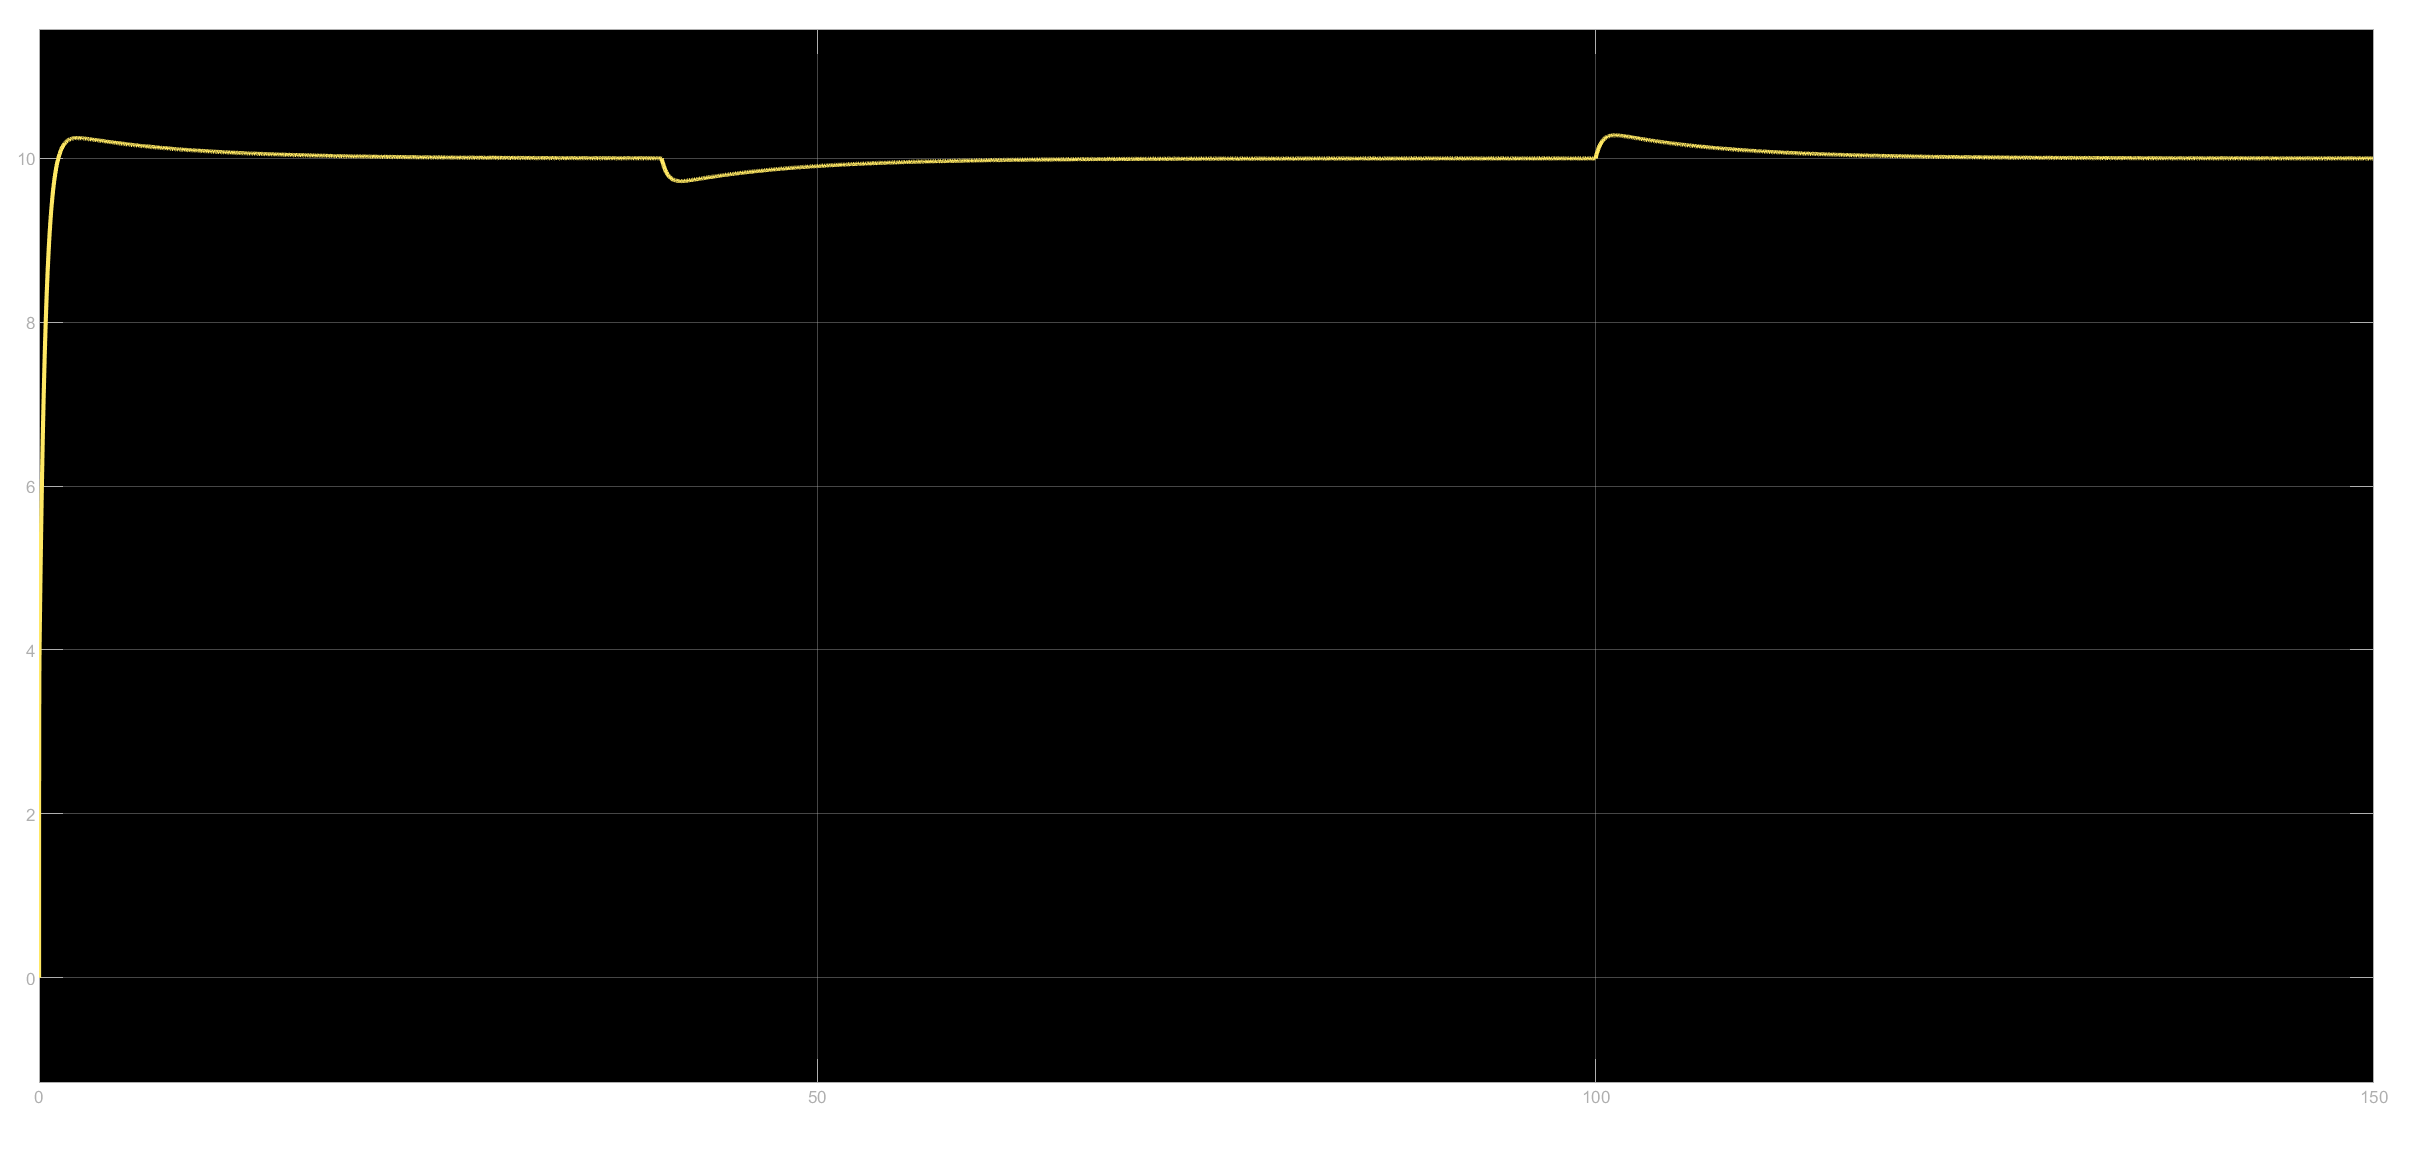
\includegraphics[ width=0.7\textwidth]{img/PID_Simulink.eps}
	\caption{پاسخ زمانی سیستم در محیط سیمولینک؛ افت سطح آب بین ثانیه ۴۰ تا ۱۰۰ ناشی از اشباع شیر ورودی در برابر اغتشاش شدید است}
	\label{pid_simulink_output}
\end{figure} 
\autoref{pid_simulink_output}
 پاسخ سیستم به این سناریو را نشان می‌دهد. نکات قابل توجه در این نمودار عبارتند از:

\begin{enumerate}
	\item \textbf{پایداری اولیه ($0 < t < 40$):} 
	سیستم با دقت بسیار بالا روی ارتفاع $10$ متر تنظیم شده و خطای حالت ماندگار صفر است.
	
	\item \textbf{رخداد اغتشاش و اشباع فیزیکی ($40 < t < 100$):} 
	در لحظه $t=40s$ با افزایش ناگهانی خروجی، سطح آب شروع به افت می‌کند.
	ولی سیستم با افزایش ورودی اب باز به سطح $10$ متر باز میگردد
	\item \textbf{بعد حذف اغتشاش}
	تا سیستم متوجه بسته شدن شیر خروجی شود و  شیر ورودی رو ببندد مقداری اب ذخیره شده و از سطح ارتفاع تعیین شده بالاتر میرود و چون موتور توانایی مکش ندارد در همان ارتفاع میماند
\end{enumerate}
\section{تحلیل اثر نویز و طراحی فیلتر جهت مقاوم‌سازی سیستم}\label{Section7}

در محیط‌های صنعتی، عواملی نظیر تلاطم سطح آب هنگام پر شدن مخزن و ارتعاشات مکانیکی، باعث ایجاد نویز روی سیگنال اندازه‌گیری شده توسط سنسور سطح می‌شوند. در این بخش، اثر این نویز بر عملکرد کنترل‌کننده و راهکارهای مقابله با آن بررسی شده است.

\subsection{شبیه‌سازی و مشاهده اثر مخرب نویز}
با افزودن یک نویز گوسی سفید $N(0, \sigma^2)$ به مسیر فیدبک، دو پدیده متفاوت مشاهده شد:
\begin{enumerate}
	\item \textbf{روی خروجی (سطح آب):} به دلیل خاصیت انتگرالی و کند بودن دینامیک مخزن (عملکرد به عنوان فیلتر پایین‌گذر طبیعی)، سطح آب تغییرات نوسانی شدیدی نشان نمی‌دهد.
	\item \textbf{روی سیگنال کنترلی (شیر ورودی):} مشکل اصلی در اینجا رخ می‌دهد. ترم مشتق‌گیر ($D$) در کنترل‌کننده PID حساسیت شدیدی به فرکانس‌های بالا دارد ($s \times Noise$). مشتق نویز باعث تولید سیگنال‌های کنترلی با دامنه بزرگ و فرکانس بالا می‌شود. این پدیده موجب باز و بسته شدن مداوم و سریع شیر شده و منجر به استهلاک مکانیکی شدید و خرابی زودرس عملگر می‌گردد
\end{enumerate}

\subsection{راهکار: فیلتر پایین‌گذر و تحلیل مصالحه 
	(\lr{Trade-off})}
برای حذف نویز فرکانس بالا، استفاده از یک فیلتر پایین‌گذر مرتبه اول ($LPF$) در مسیر فیدبک پیشنهاد می‌شود:
\begin{equation}
	H_{filter}(s) = \frac{1}{T_f s + 1}
\end{equation}
که در آن $T_f$ ثابت زمانی فیلتر است. افزودن این فیلتر یک چالش اساسی بین «کیفیت حذف نویز» و «پایداری سیستم» ایجاد می‌کند:

\begin{itemize}
	\item \textbf{مزیت (حذف نویز):} فیلتر با تضعیف فرکانس‌های بالا، سیگنال ورودی به مشتق‌گیر را هموار کرده و از لرزش شیر جلوگیری می‌کند.
	\item \textbf{عیب (تأخیر فاز):} فیلتر پایین‌گذر ذاتاً باعث ایجاد تأخیر فاز (\lr{Phase Lag}) در حلقه کنترلی می‌شود. زاویه فاز اضافه شده برابر است با $\phi = -\arctan(\omega T_f)$.
	\item \textbf{تحلیل پایداری:} این تأخیر فاز مستقیماً از \textbf{حاشیه فاز (\lr{Phase Margin})} سیستم می‌کاهد. اگر $T_f$ بیش از حد بزرگ انتخاب شود (فیلترینگ سنگین)، حاشیه فاز به سمت صفر میل کرده و سیستم ناپایدار می‌شود.
\end{itemize}

\textbf{نتیجه‌گیری طراحی:} مقدار $T_f$ باید به گونه‌ای انتخاب شود که نویز را حذف کند اما فرکانس قطع آن ($1/T_f$) بسیار بزرگتر از پهنای باند سیستم کنترلی باشد تا دینامیک اصلی سیستم را کند نکند.

\section{بررسی امکان‌پذیری کاهش ثابت زمانی به یک ثانیه}\label{Section8}

ثابت زمانی ذاتی سیستم مخزن در حال حاضر حدود $\tau \approx 221$ ثانیه است. کاهش این مقدار به ۱ ثانیه (افزایش سرعت سیستم به میزان ۲۲۰ برابر) نیازمند تغییرات بنیادین در پارامترهای فیزیکی یا استراتژی کنترلی است.

\subsection{تحلیل تغییرات پارامترهای فیزیکی}
ثابت زمانی سیستم حلقه باز از رابطه $\tau = \frac{2A}{a\sqrt{2g}}$ بدست می‌آید. برای اینکه $\tau \to 1s$ شود، باید صورت کسر کوچک یا مخرج آن بسیار بزرگ شود:
\begin{enumerate}
	\item \textbf{تغییر ابعاد مخزن ($A$):} سطح مقطع مخزن باید حدود ۲۲۰ برابر کوچکتر شود. این یعنی تبدیل مخزن به یک لوله باریک عمودی. در این حالت ظرفیت ذخیره‌سازی از دست می‌رود.
	\item \textbf{تغییر خروجی ($a$):} مساحت دریچه خروجی باید ۲۲۰ برابر بزرگتر شود. این یعنی عملاً کف مخزن کاملاً باز باشد که دیگر مخزن نخواهد بود.
\end{enumerate}
\textbf{نتیجه:} تغییر فیزیکی برای رسیدن به این عدد غیرعملی است.

\subsection{تحلیل تغییرات کنترلی }
در روش کنترلی، ما با استفاده از فیدبک قوی، مکان قطب‌های حلقه بسته را جابجا می‌کنیم. اگر بخواهیم ثابت زمانی حلقه بسته ۱ ثانیه باشد، باید قطب غالب سیستم در $s = -1$ قرار گیرد.
تقریب معادله مشخصه با کنترل‌کننده تناسبی ($K_p$) برابر است با:
\begin{equation}
	s + (a_{sys} + K_p K_{plant}) = 0 \quad \Rightarrow \quad a_{sys} + 0.01 K_p = 1
\end{equation}
با حل این معادله، بهره تناسبی مورد نیاز حدود $K_p \approx 100$ بدست می‌آید.

\subsubsection{چالش اصلی: محدودیت انرژی 
	\lr{(Actuator Saturation)}}
اگرچه روی کاغذ با $K_p=100$ می‌توان به ثابت زمانی ۱ ثانیه رسید، اما در عمل با یک مانع فیزیکی روبرو هستیم:
برای اینکه سطح آب تانکر در ۱ ثانیه به مقدار مطلوب برسد، حجم عظیمی از آب باید در یک لحظه وارد مخزن شود.
\begin{equation}
	Q_{in} = A \times \frac{dh}{dt} \approx 100 \times \frac{1m}{1s} = 100 \, m^3/s
\end{equation}
تأمین دبی $100$ متر مکعب بر ثانیه نیازمند پمپ‌های صنعتی غول‌پیکر و لوله‌های بسیار قطور است. شیر ورودی فعلی بلافاصله 
\textbf{اشباع}
 شده و سیستم عملاً نمی‌تواند سریع‌تر از نرخ حداکثر جریان شیر پر شود.
بنابراین، رسیدن به ثابت زمانی ۱ ثانیه تنها با تغییر کنترل‌کننده امکان‌پذیر نیست و نیازمند تغییر سخت‌افزاری (پمپ و شیر بسیار قوی‌تر) است.


\newpage
\href{https://github.com/MJAHMADEE/ARASLaTeXFormats}{گیتهاب (\lr{GitHub})}.

\end{document}
